\documentclass[12pt]{article}

%\usepackage{mathptm}  
\usepackage{a4}
\usepackage{hyperref}
\usepackage{color}
\usepackage{graphicx}
\usepackage{fancyhdr}
\usepackage{multicol}
\usepackage{amstext}
\usepackage{amsmath}
%\usepackage{fullpage}
%\usepackage{parskip}
\usepackage[colon]{natbib}
%\usepackage{rotating}
\usepackage{pdflscape}
\usepackage{longtable}
\usepackage{caption}
\usepackage{subcaption}
%\usepackage[nomarkers,figuresonly]{endfloat}
\usepackage{amsfonts}
\usepackage{pifont}
\usepackage{authblk}
\usepackage{epstopdf}
\usepackage{multirow}
\usepackage{amsfonts}

\textwidth 160mm
\textheight 235mm
\oddsidemargin 0mm
\topmargin -15mm
\baselineskip 13pt
\parskip 1pc
\parindent 0pc

\pagestyle{fancy}
\cfoot{\thepage}

\renewcommand{\headrulewidth}{0.2pt}
\renewcommand{\footrulewidth}{0.2pt}

\newcommand\Bo{\mbox{\textit{Bo}}}  % Bond number
\newcommand\Ca{\mbox{\textit{Ca}}} %Capillary number

\definecolor{darkred}{rgb}{0.80,0.00,0.05}
\definecolor{blue}{rgb}{0.00,0.00,0.95}
\definecolor{darkgreen}{rgb}{0.00,0.60,0.0}
\definecolor{gray}{rgb}{0.95,0.9,0.9}

\usepackage{listings}
\lstset{language=C++}
\lstset{backgroundcolor=\color{gray}}
\lstset{breaklines=true}
\lstset{basicstyle=\ttfamily\small}
\lstset{showstringspaces=false}
\lstset{keywordstyle=\color{blue}\bfseries}
\lstset{commentstyle=\ttfamily\small\color{darkgreen}}
\lstset{identifierstyle=\color{darkred}\bfseries}
\lstset{numbers=left,numberstyle=\tiny}
\lstset{columns=fixed,basewidth=0.45em}

\DeclareMathOperator\erf{erf}

\linespread{1.5}

\begin{document}
\thispagestyle{empty}

\title{Low Reynolds number gravitational settling of a sphere through a fluid-fluid interface: Modelling using a boundary integral method}

\author[1]{Paul Jarvis\footnote{Corresponding author:paul.jarvis@bristol.co.uk}}
\author[1]{Jon Blundy}
\author[1]{Katharine Cashman}
\author[1,2]{Herbert E Huppert}
\author[1]{Heidy Mader}
\affil[1]{\small School of Earth Sciences, University of Bristol, Wills Memorial Building, Queens Road, Bristol, BS8 1RJ, UK}
\affil[2]{\small Department of Applied Mathematics and Theoretical Physics, University of Cambridge, Wilberforce Road, Cambridge, CB3 0WA, UK}
\date{}
% NOTE: A full address must be provided: department, university/institution, town/city, zipcode/postcode, country.


\maketitle

\begin{abstract}


\end{abstract}


\section{Introduction}
\label{sec:intro}


\section{Theoretical Background}
\label{sec:theory}

We present a theoretical construction of the boundary integral equations. Symbols used are defined in table~\ref{tab:symbols}.

    \begin{longtable}{|c|c|}
    \caption{Definition of symbols. \label{tab:symbols}} \\ % title name of the table
    \hline
    Symbol & Definition \\  
    \hline % inserts single-line
    $a$                                                               & Sphere radius           \\
    $f_{\text{s},i}(\mathbf{x}) = m_{j}(\mathbf{x})T_{1,ij}(\mathbf{x})$   &Traction on surface of sphere \\
    $f_{\alpha,i}(\mathbf{x}) = n_{j}(\mathbf{x})T_{\alpha,ij}(\mathbf{x})$ & Traction of fluid $\alpha$ on interface \\
    $\mathcal{F}_{i}$                                                  & Arbitrary constant vector \\
    $\boldsymbol{F}$                                                  & Force vector \\
    $\mathbf{g} = (-9.81 \text{m s}^{-2}) \mathbf{\hat{z}}$            & Acceleration due to gravity \\      
    $\mathcal{I}$                                                     & Surface of interface \\
    $m$                                                               & Outward normal to sphere surface \\
    $n$                                                               & Normal to interface (points into fluid 1) \\
    $p_{\alpha}(\mathbf{x})$                                            & Pressure field of fluid $\alpha$ \\
    $p_{\text{d},\alpha}(\mathbf{x}) $                                    & Dynamic pressure of fluid $\alpha$ \\
    $s$                                                               & Arc length along interface measured from axis \\
    $\mathcal{S}$                                                     & Surface of sphere \\
    $T_{\alpha,ij}(\mathbf{x})$                                          & Stress tensor field of fluid $\alpha$ \\
    $\hat{T}_{\alpha,ij}(\boldsymbol{x'} - \boldsymbol{y'})$             & Stress Greens function for fluid $\alpha$ \\
    $t$                                                               & Time \\
    $\mathbf{u}_{\alpha}(\mathbf{x})$                                   & Velocity field of fluid $\alpha$ \\
    $\mathbf{u}_{\text{s}} = u_{\text{s}} \mathbf{\hat{z}}$                & Velocity of sphere \\
    $\hat{u}_{\alpha,i}(\boldsymbol{x'} - \boldsymbol{y'})$              & Velocity Greens function for fluid $\alpha$ \\
    $\mathcal{V}_{\alpha}$                                              & Volume of fluid $\alpha$ \\
    $\mathbf{x}$                                                      & Position vector \\
    $\mathbf{y}$                                                      & Position vector \\
    $\mathbf{\hat{z}}$                                                & Unit vector in the upward vertical direction \\
    $\alpha = 1,2$                                                    & Fluid label \\
    $\delta_{ij} = \begin{cases}
    1  & \quad \text{if } i = j\\
    0  & \quad \text{if } i \neq j\\
  \end{cases}$                                                        & Kronecker delta \\
    $\delta(\boldsymbol{x'} - \boldsymbol{y'}) = \begin{cases}
    1  & \quad \text{if } \boldsymbol{x} = \boldsymbol{y}\\
    0  & \quad \text{if } \boldsymbol{x} \neq \boldsymbol{y}\\
  \end{cases}$                                                        & Dirac delta function \\
    $\eta_{\alpha}$                                                     & Viscosity of fluid $\alpha$ \\ 
    $\theta$                                                          & Polar angle with respect to sphere centre \\
    $\rho_{\alpha}$                                                     & Density of fluid $\alpha$   \\
    $\rho_{\text{s}}$                                                   & Sphere density          \\
    $\sigma$                                                          & Interfacial Tension     \\
    $\phi$                                                            & Azimuhtal angle with respect to axis of motion \\
    \hline % inserts single-line
  \end{longtable}

\subsection{Equations of Motion}
\label{subsec:EoM}

The starting point for all fluid dynamical problems are the continuity (equation~\ref{equ:full_cont}) and Navier Stokes (equation~\ref{equ:NS_comp}) equations \citep{Batchelor67}:

\begin{equation}
\label{equ:full_cont}
\frac{\partial \rho_{\alpha}(\boldsymbol x,t)}{\partial t} + \boldsymbol\nabla \cdot [\rho_{\alpha}(\boldsymbol{x},t) \boldsymbol{u}_{\alpha} (\boldsymbol{x},t)] = 0 ,
\end{equation}  

\begin{equation}
\label{equ:NS_comp}
\begin{array}{l}
\rho_{\alpha}(\boldsymbol{x},t) \left( \frac{\partial \boldsymbol{u}_{\alpha}(\boldsymbol{x},t)}{\partial t} + (\boldsymbol{u}_{\alpha}(\boldsymbol{x},t) \cdot \boldsymbol\nabla) \boldsymbol{u}_{\alpha}(\boldsymbol{x},t) \right) = \\[5pt]
- \boldsymbol\nabla P_{\alpha}(\boldsymbol{x},t) - \rho_{\alpha}(\boldsymbol{x},t) g + \eta_{\alpha} \left[\nabla^{2} \boldsymbol{u}_{\alpha}(\boldsymbol{x},t) + \frac{\boldsymbol\nabla(\boldsymbol\nabla \cdot \boldsymbol{u}_{\alpha}(\boldsymbol{x},t))}{3} \right] .
\end{array}
\end{equation} 

Forming a coupled set of non-linear, partial differential equations for the velocity and pressure fields, these represent mass and momentum conservation respectively and must be satisfied by all fluid phases within the system. For most practical applications, the fluids are assumed to be incompressible (have constant density) and so the continuity equation reduces to the incompressibility relation

\begin{equation}
\label{equ:incom}
\boldsymbol\nabla \cdot \boldsymbol{u}_{\alpha}(\boldsymbol{x},t) = 0 .
\end{equation}

This can be combined with equation~\ref{equ:NS_comp} to form the incompressible Navier Stokes equation

\begin{equation}
\label{equ:NS_incom}
\rho_{\alpha} \left( \frac{\partial \boldsymbol{u}_{\alpha}(\boldsymbol{x},t)}{\partial t} + (\boldsymbol{u}_{\alpha}(\boldsymbol{x},t) \cdot \boldsymbol\nabla) \boldsymbol{u}_{\alpha}(\boldsymbol{x},t) \right) = - \boldsymbol\nabla P_{\alpha}(\boldsymbol{x},t) - \rho_{\alpha} g + \eta_{\alpha} \nabla^{2} \boldsymbol{u}_{\alpha}(\boldsymbol{x},t) .
\end{equation} 

The equations of motion can be expressed in an alternative form by defining the stress tensor $\boldsymbol{T}_{\alpha}(\boldsymbol{x},t)$ \citep{Manga94} and dynamic pressure $P_{\text{d},\alpha}(\boldsymbol{x},t)$:

\begin{equation}
\label{equ:stress}
\boldsymbol{T}_{\alpha}(\boldsymbol{x},t) = -P_{\text{d},\alpha}(\boldsymbol{x},t)  \boldsymbol{I} + \eta_{\alpha}[\boldsymbol\nabla \boldsymbol{u}_{\alpha}(\boldsymbol{x},t) + (\boldsymbol\nabla \boldsymbol{u}_{\alpha}(\boldsymbol{x},t))^{T}], 
\end{equation}

\begin{equation}
\label{equ:dyn_P}
P_{\text{d},\alpha}(\boldsymbol{x},t) = P_{\alpha}(\boldsymbol{x},t) - \rho_{\alpha} \boldsymbol{g} \cdot \boldsymbol{x} .
\end{equation}

This definition of the stress tensor removes the gravitational body force from the equations of motion, meaning that it only appears in the boundary conditions. The Navier Stokes equation then becomes

\begin{equation}
\label{equ:NS_stress}
\rho_{\alpha} \left( \frac{\partial \boldsymbol{u}_{\alpha}(\boldsymbol{x},t)}{\partial t} + (\boldsymbol{u}_{\alpha}(\boldsymbol{x},t) \cdot \boldsymbol\nabla) \boldsymbol{u}_{\alpha}(\boldsymbol{x},t) \right) = \boldsymbol\nabla \cdot \boldsymbol{T}_{\alpha}(\boldsymbol{x},t) .
\end{equation}

When working in fluid dynamics, it is usual to non-dimensionalise the equations of motion and boundary conditions \citep{White99}. This can be achieved by scaling the quantities involved by parameters specific to the problem. For example, consider a problem with typical scales of length $L_{\text{c}}$ and velocity $U_{\text{c}}$. This allows us to define dimensionless variables (denoted by a $'$)

\begin{equation} 
\label{equ:nodim_l}
\boldsymbol{x} = L_{\text{c}} \boldsymbol{x'} ,
\end{equation}

\begin{equation}
\label{equ:nodim_u}
\boldsymbol{u}_{\alpha}(\boldsymbol{x},t) = U_{\text{c}} \boldsymbol{u'}_{\alpha}(\boldsymbol{x'},t') ,
\end{equation}

and 

\begin{equation}
\label{equ:nodim_t}
t = \frac{L_{\text{c}} t'}{U_{\text{c}}}
\end{equation}

In the case of highly viscous flows, the pressure is dominated by viscosity and so the relevant scaling for the dynamic pressure uses a characteristic viscosity $\eta_{\text{c}}$ and is given by\citet{Lee82}

\begin{equation}
\label{equ:nodim_p_highRE}
P_{\text{d},\alpha}(\boldsymbol{x},t) = \frac{\eta_{\text{c}} U_{\text{c}} P_{\text{d},\alpha}'(\boldsymbol{x'},t')}{L_{\text{c}}} .
\end{equation}

This choice of pressure scaling means that upon substitution of equations~\ref{equ:nodim_l} to~\ref{equ:nodim_p_highRE} into equation~\ref{equ:stress} the stress tensor can also be non-dimensionalised,

\begin{equation}
\label{equ:nodim_T}
\boldsymbol{T}_{\alpha}(\boldsymbol{x},t) = \frac{\eta_{\text{c}} U_{\text{c}} \boldsymbol{T'}_{\alpha}(\boldsymbol{x'},t')}{L_{\text{c}}} \quad \text{where} \quad \boldsymbol{T'}_{\alpha}(\boldsymbol{x'},t') = p_{\text{d},\alpha}'(\boldsymbol{x'},t') \boldsymbol{I} + \frac{\eta_{\alpha} [\boldsymbol\nabla' \boldsymbol{u'}_{\alpha}(\boldsymbol{x'},t') + (\boldsymbol\nabla' \boldsymbol{u'}_{\alpha}(\boldsymbol{x'},t'))^{T}]}{\eta_{c}} .
\end{equation}

In this case, the continuity and Navier Stokes equations become

\begin{equation}
\label{equ:nodim_cont}
\boldsymbol\nabla' \cdot \boldsymbol{u'}_{\alpha}(\boldsymbol{x'},t') = 0
\end{equation}

and

\begin{equation}
\label{equ:NS_low_Reynolds}
\text{Re} \left(\frac{\partial \boldsymbol{u'}_{\alpha}(\boldsymbol{x'},t')}{\partial t'} + (\boldsymbol{u'}_{\alpha}(\boldsymbol{x'},t') \cdot \boldsymbol\nabla') \boldsymbol{u'}_{\alpha}(\boldsymbol{x'},t') \right) = \boldsymbol\nabla' \cdot \boldsymbol{T'}_{\alpha}(\boldsymbol{x'},t') ,
\end{equation}

where the Reynolds number is defined as

\begin{equation}
\label{equ:Reynolds}
\text{Re}_{\alpha} = \frac{\rho_{\alpha} L_{\text{c}} U_{\text{c}}}{\eta_{\text{c}}}
\end{equation}

As we are considering the case of low Reynolds number ($\text{Re}_{\alpha} \ll 1$), we can neglect the inertial terms on the right hand side and the equation reduces to the Stokes equation \cite{Kim05}

\begin{equation}
\label{equ:Stokes}
\boldsymbol{\nabla'} \cdot \boldsymbol{T'}_{\alpha}(\boldsymbol{x'},t') = \boldsymbol{0} .
\end{equation}


\subsection{Boundary Conditions}
\label{subsec:BC}

In order to complete the formulation of any fluid dynamics problem, it is necessary to state the boundary conditions alongside the equations of motion \citep{Riley06}. For fluids of infinite (or semi-infinite) extent in some dimension, these include the value of the flow velocity at infinity. For bounded flows, the conditions are imposed at the boundaries of the fluid domain, and their exact nature depends on the phase of the material bounding it.

\subsubsection{Fluid-Solid Boundary}
\label{subsubsec:BC_fluid-solid}

At low Reynolds number for a fluid-solid boundary given by the surface $\mathcal{S}$ (see figure~\ref{fig:fluid-solid_boundary}), the kinematic boundary condition (that on the velocity) states that both the normal and tangential components (with respect to the boundary) of velocity are the same as that of the solid at the boundary. This is easily expressed in dimensionless form as

\begin{equation}
\label{equ:lowRE_fluid-solid}
\boldsymbol{u'}_{\alpha}(\boldsymbol{x'}) = \boldsymbol{U}_{\text{s}}' \quad \boldsymbol{x} \in \mathcal{S} .
\end{equation}

\begin{figure}
$$\includegraphics[width=80mm]{fluid_solid.eps}$$
\caption{Definition of $\boldsymbol{m}$ and $\mathcal{S}$ for a fluid-solid boundary. \label{fig:fluid-solid_boundary}}
\end{figure}

There also needs to be a dynamic boundary condition applied at the interface. If the solid exerts a force $\boldsymbol{F}$ onto the fluid then the condition states

\begin{equation}
\label{equ:dyn_fluid_solid}
\int \boldsymbol{m} \cdot \boldsymbol{T}_{\alpha} \mathrm{d} \mathcal{S} = \boldsymbol{F} .
\end{equation}

Using the non-dimensionalisation scheme presented above this becomes

\begin{equation}
\label{equ:nodim_fluid_solid}
\eta_{\text{c}} U_{\text{c}} L_{\text{c}} \int \boldsymbol{m} \cdot \boldsymbol{T'}_{\alpha} \mathrm{d} \mathcal{S'} = \boldsymbol{F} .
\end{equation}

\subsubsection{Fluid-Fluid Boundary}
\label{subsubsec:BC_fluid-fluid}

In the case of a fluid-fluid boundary (see figure~\ref{fig:fluid-fluid_boundary}), both a kinematic and dynamic boundary condition need to be satisfied. The kinematic boundary condition states that the velocity of the two fluids must be continuous across the interface \citep{Manga94}. Expressed in dimensionless form this looks like

\begin{equation}
\label{equ:fluid_fluid_kin}
\boldsymbol{u'}_{1}(\boldsymbol{x'}) = \boldsymbol{u'}_{2}(\boldsymbol{x'}), \quad \boldsymbol{x'} \in \mathcal{I} .
\end{equation}

\begin{figure}
$$\includegraphics[width=80mm]{fluid_fluid.eps}$$
\caption{Definition of $\boldsymbol{n}$ and $\mathcal{I}$ for a fluid-fluid boundary. \label{fig:fluid-fluid_boundary}}
\end{figure}

The dynamic boundary condition is an expression of the balance between the stress discontinuity across the interface and the interfacial tension (IFT)\citep{Manga94}:

\begin{equation}
\label{equ:fluid_fluid_dyn}
\boldsymbol{n} \cdot [\boldsymbol{T}_{1} (\boldsymbol{x}) - \rho_{1}(\boldsymbol{g} \cdot \boldsymbol{x}) \boldsymbol{I}] - \boldsymbol{n} \cdot [\boldsymbol{T}_{2} (\boldsymbol{x}) - \rho_{2} (\boldsymbol{g} \cdot \boldsymbol{x}) \boldsymbol{I}] = \sigma(\boldsymbol{x}) \boldsymbol{n} (\boldsymbol{\nabla}_{\text{s}} \cdot \boldsymbol{n}) - \boldsymbol{\nabla}_{\text{s}} \sigma (\boldsymbol{x}) , \quad \boldsymbol{x} \in \mathcal{I} .
\end{equation}

The operator $\boldsymbol{\nabla}_{\text{s}}$ is defined as the tangential gradient operator within the surface $\mathcal{I}$:

\begin{equation}
\label{equ:surf_grad}
\boldsymbol{\nabla}_{\text{s}} = (\boldsymbol{I} - \boldsymbol{n} \boldsymbol{n}) \cdot \boldsymbol{\nabla} .
\end{equation}

When this takes the normal vector as its argument it can be shown that \citep{Brackbill92}

\begin{equation}
\label{equ:tang_diff_norm}
\boldsymbol{\nabla}_{\text{s}} \cdot \boldsymbol{n} = \boldsymbol{\nabla} \cdot \boldsymbol{n}.
\end{equation}

The presence of gradients in the interfacial tension can lead to so-called Marangoni effects \citep{Kim05}. However, for present purposes we will assume that the interfacial tension is uniform across the interface S and so the last term on the right hand side equals zero;

\begin{equation}
\label{equ:fluid_fluid_dyn_nograd}
\boldsymbol{n} \cdot [\boldsymbol{T}_{1} (\boldsymbol{x}) - \rho_{1} (\boldsymbol{g} \cdot \boldsymbol{x}) \boldsymbol{I}] - \boldsymbol{n} \cdot [\boldsymbol{T}_{2} (\boldsymbol{x}) - \rho_{2} (\boldsymbol{g} \cdot \boldsymbol{x}) \boldsymbol{I}] = \sigma(\boldsymbol{x}) \boldsymbol{n} (\boldsymbol{\nabla} \cdot \boldsymbol{n}),  \quad \boldsymbol{x} \in \mathcal{S}.
\end{equation}

Like the equations of motion, this can be non-dimensionalised using equations~\ref{equ:nodim_l} to~\ref{equ:nodim_T}:

\begin{equation}
\label{equ:nodim_fluid_fluid_dyn}
\text{Ca } \boldsymbol{n} \cdot (\boldsymbol{T'}_{1} - \boldsymbol{T'}_{2}) + \text{Bo}(\boldsymbol{\hat{z}} \cdot \boldsymbol{x'}) \boldsymbol{n} = (\boldsymbol{\nabla'} \cdot \boldsymbol{n}) \boldsymbol{n}.
\end{equation}

The capillary number $\text{Ca}$ and  Bond number $\text{Bo}$ are dimensionless numbers defined as:

\begin{equation}
\label{equ:cap}
\text{Ca} = \frac{\eta_{\text{c}} U_{\text{c}}}{\sigma}
\end{equation}

\begin{equation}
\label{equ:Bond}
\text{Bo} = \frac{(\rho_{2} - \rho_{1}) g L_{\text{c}}^{2}}{\sigma}
\end{equation}

The $\mathbf{\nabla} \cdot \mathbf{n}$ factor in equation~\ref{equ:fluid_fluid_dyn} can be expressed in a more physically meaningful manner by noting that it is related to the mean curvature, $K$, of the interface \citep{Hobson11}.

\begin{equation}
\label{equ:surf_curv}
2 K = -\mathbf{\nabla} \cdot \mathbf{n}
\end{equation}


\subsection{Problem Statement}
\label{subsec:theory}

The system is formulated as in figure~\ref{fig:params}. The physical parameters motivate the choice of scaling variables. The characteristic lengthscale is chosen to be the sphere radius $a$, characteristic viscosity that of the upper fluid $\eta_{1}$ and characteristic velocity to be the Stokes velocity \citep{Reynolds1886},

\begin{equation}
\label{equ:char_vel}
U_{\text{c}} = \frac{2 (\rho_{\text{s}} - \rho_{1}) g a^{2}}{9 \eta_{1}} .
\end{equation}

  \begin{figure}
    $$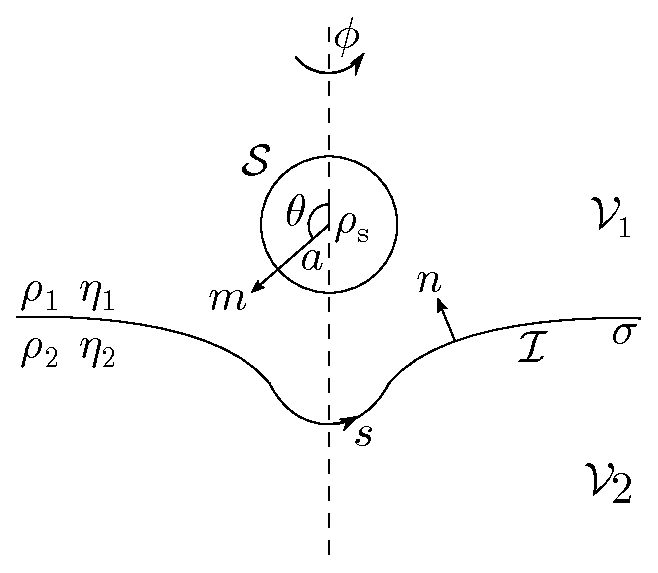
\includegraphics[width=0.8\textwidth]{formulation.eps}$$
    \caption{Diagrammatic representation of the system. A sphere falls under gravity, at low Reynolds number, towards an initially horizontal interface between two density stratified, immiscible semi-infinite fluids. See table~\ref{tab:symbols} for definition of symbols. \label{fig:params}}
  \end{figure}

This means the capillary and Bond numbers can be expressed as:

\begin{equation}
\label{equ:cap_spec}
\text{Ca} = \frac{(\rho_{\text{s}} - \rho_{1}) g a^{2}}{\sigma},
\end{equation}

\begin{equation}
\label{equ:bond_spec}
\text{Bo} = \frac{(\rho_{2} - \rho_{1}) g a^{2}}{\sigma}.
\end{equation}

The dimensionless stress tensor for each fluid can be written as

\begin{equation}
\label{equ:nd_stress_def}
T_{\alpha, ij}'(\boldsymbol{x'}) = -P_{\text{d,} \alpha}'(\boldsymbol{x'}) \delta_{ij} + \Lambda_{\alpha}[\partial_{i}' u_{\alpha, j}'(\boldsymbol{x'}) - \partial_{j}' u_{\alpha, i}'(\boldsymbol{x'})].
\end{equation}

The parameter $\Lambda_{\alpha}$ is defined as

\begin{equation}
\label{equ:Llambda}
\Lambda_{\alpha} = \frac{\eta_{\alpha}}{\eta_{1}} = \left\{
    \begin{array}{l l}
      1, & \quad \alpha = 1 \\
      \frac{\eta_{2}}{\eta_{1}} = \lambda, & \quad \alpha = 2
    \end{array} \right.\ .
\end{equation}

Note $\lambda$ is the viscosity ratio of the two fluids. It is straightforward to apply the general equations of motion and boundary conditions to the problem. The equations of motion, expressed in the Einstein summation convention \citep{Riley06} which will be used from now on, appear as 

\begin{equation}
\label{equ:cont}
\partial_{\text{i}}' u_{\alpha,i}'(\boldsymbol{x'}) = 0,
\end{equation}

and 

\begin{equation}
\label{equ:stokes}
\partial_{\text{i}}' T_{\alpha,ij}'(\boldsymbol{x'}) = 0.
\end{equation}

Here, $\alpha = 1,2$ and denotes the fluid, $i, j$ denote components of tensoral quantities. 

The first boundary condition that we impose is that the undisturbed fluid is quiescent;

\begin{equation}
\label{equ:BC_inf}
u_{\alpha, i}'(\boldsymbol{x'}) \to 0 \text{ as } |\boldsymbol{x'}| \to \infty.
\end{equation}

The kinematic boundary condition on the fluid interface (equation~\ref{equ:fluid_fluid_kin}) can be expressed as  

\begin{equation}
\label{equ:BC_kin_int_nodim}
u_{1,i}'(\boldsymbol{x'}) = u_{2,i}'(\boldsymbol{x'}), \quad \boldsymbol{x'} \in S_{\text{int}}.
\end{equation}

The dynamic boundary condition is also imposed at the interface;

\begin{equation}
\label{equ:BC_dyn_int}
\text{Ca } n_{i} [T_{1, ij}'(\boldsymbol{x'}) - T_{2,ij}'(\boldsymbol{x'})] + \text{Bo} \hat{z}_{i} x_{i}' n_{j} = n_{j} \partial_{i}' n_{i}.
\end{equation}

The kinematic boundary condition on the sphere surface is one of no-slip meaning the fluid velocity at the surface has to equal the sphere velocity ;

\begin{equation}
\label{equ:BC_kin_spere}
u_{1,i}'(\boldsymbol{x'}) = u_{\text{s},i}', \quad \boldsymbol{x'} \in \mathcal{S}.
\end{equation}

The final boundary condition is the dynamic boundary condition on the sphere. The force on the fluid due to the sphere originates from the balance between gravity and buoyancy;

\begin{equation}
\label{equ:sphere_force}
F_{i} = \frac{- 4 \pi a^{3} (\rho_{\text{s}} - \rho_{1}) g \hat{z}_{i}}{3}.
\end{equation}

Substituting this into equation~\ref{equ:nodim_fluid_solid} and using equation~\ref{equ:char_vel} we obtain

\begin{equation}
\label{equ:BC_dyn_sphere}
\int_{\mathcal{S}} n_{i} T_{1, ij}'(\boldsymbol{x'}) \mathrm{d} \mathcal{S}' = \frac{-4 \pi \hat{z}_{i}}{3}
\end{equation}

The dimensionless numbers that describe the system are the set $\{\lambda, \text{Ca}, \text{Bo}\}$. However, an equivalent set can be generated by defining the dimensionless density ratio $D$;

\begin{equation}
\label{equ:dim_dens_rat}
D = \frac{\text{Ca}}{\text{Bo}} = \frac{\rho_{\text{s}} - \rho_{1}}{\rho_{2} - \rho_{1}}.
\end{equation}

Therefore, we can also describe the system with the set $\{\lambda, D, \text{Bo}\}$. This allows us to re-express equation~\ref{equ:BC_dyn_int} as

\begin{equation}
\label{equ:d_int}
D \text{Bo } n_{i} [T_{1, ij}'(\boldsymbol{x'}) - T_{2, ij}'(\boldsymbol{x'})] = n_{j}(\partial_{i}' n_{i} - \text{Bo} \hat{z}_{i} x_{i}')
\end{equation}

To summarise, the problem is completely described by equations~\ref{equ:cont} to~\ref{equ:BC_kin_int_nodim}, and equations~\ref{equ:BC_kin_spere},~\ref{equ:BC_dyn_sphere} and~\ref{equ:d_int}.


\subsection{Greens functions}
\label{subsec:BIE_deriv}

In order to derive the boundary integral equations, it is necessary to make use of the Greens functions for Stokes flow, $\hat{u}_{\alpha,i}(\boldsymbol{x'} - \boldsymbol{y'})$ and $\hat{T}_{\alpha,ij}(\boldsymbol{x'} - \boldsymbol{y'})$, defined such that

\begin{equation}
\label{equ:vel_green_def}
\partial' \hat{u}_{\alpha,i}(\boldsymbol{x'} - \boldsymbol{y'}) = 0 
\end{equation}

and

\begin{equation}
\label{equ:stress_green_def}
\partial' \hat{T}_{\alpha,ij}(\boldsymbol{x'} - \boldsymbol{y'}) + \mathcal{F}_{j} \delta(\boldsymbol{x'} - \boldsymbol{y'}) = 0 .
\end{equation}

Equations~\ref{equ:vel_green_def} and~\ref{equ:stress_green_def} can be solved using Fourier transforms (appendix INSERT REF HERE) to show that


\bibliographystyle{plainnat}

\bibliography{bim_bib}


\end{document}